\documentclass[a4paper,10pt]{article}
\usepackage[margin=2.5cm]{geometry}

\usepackage{amssymb,amsmath,amsthm}
\usepackage{color}
\usepackage{enumitem}
\usepackage{dsfont}
\usepackage{bm}


\newtheorem{theorem}{Theorem}
\newtheorem{proposition}{Proposition}
\newtheorem{cor}{Corollary}
\theoremstyle{definition}
\newtheorem{definition}{Definition}
\newtheorem{remark}{Remark}
\newtheorem{example}{Example}
\newtheorem{claim}{Claim}
\newtheorem{lemma}{Lemma}


%%%%%%%%%%%%%%%%%%%%%%%%%%%%%%%%%%%%%%%%%%%%%%%%%%%%%%%%%%%%%%%%%%%%%%%%%%%%%%%
% Algorithms
%%%%%%%%%%%%%%%%%%%%%%%%%%%%%%%%%%%%%%%%%%%%%%%%%%%%%%%%%%%%%%%%%%%%%%%%%%%%%%%

\usepackage{algorithm}
\usepackage{algorithmic}
\usepackage[titlenumbered,ruled,noend,algo2e]{algorithm2e}
\newcommand\mycommfont[1]{\footnotesize\ttfamily\textcolor{blue}{#1}}
\SetCommentSty{mycommfont}
\SetEndCharOfAlgoLine{}


%%%%%%%%%%%%%%%%%%%%%%%%%%%%%%%%%%%%%%%%%%%%%%%%%%%%%%%%%%%%%%%%%%%%%%%%%%%%%%%
% Code
%%%%%%%%%%%%%%%%%%%%%%%%%%%%%%%%%%%%%%%%%%%%%%%%%%%%%%%%%%%%%%%%%%%%%%%%%%%%%%%


\usepackage{fancyvrb}                  % for fancy verbatim
\usepackage{textcomp}
\usepackage[space=true]{accsupp}
% requires the latest version of package accsupp
\newcommand{\copyablespace}{
    \BeginAccSupp{method=hex,unicode,ActualText=00A0}
\ %
    \EndAccSupp{}
}
\usepackage[procnames]{listings}
% \usepackage{setspace} % need for \setstretch{1}
\lstset{%
language   = python,%
 % basicstyle = \ttfamily\setstretch{1},%
basicstyle = \ttfamily,%
columns    = flexible,%
keywordstyle=\color{javared},
firstnumber=100,
frame=shadowbox,
showstringspaces=false,
morekeywords={import,from,class,def,for,while,if,is,in,elif,
else,not,and,or,print,break,continue,return,True,False,None,access,
as,del,except,exec,finally,global,import,lambda,pass,print,raise,try,assert,!=},
keywordstyle={\color{javared}\bfseries},
commentstyle=\color{javagreen}, %vsomb_col white comments
morecomment=[s][\color{javagreen}]{"""}{"""},
upquote=true,
%% style for number
numbers=none,
resetmargins=true,
xleftmargin=10pt,
linewidth= \linewidth,
numberstyle=\tiny,
stepnumber=1,
numbersep=8pt, %
frame=shadowbox,
rulesepcolor=\color{black},
procnamekeys={def,class},
procnamestyle=\color{oneblue}\textbf,
literate={á}{{\'a}}1
{à}{{\`a }}1
{ã}{{\~a}}1
{é}{{\'e}}1
{ê}{{\^e}}1
{è}{{\`e}}1
{í}{{\'i}}1
{î}{{\^i}}1
{ó}{{\'o}}1
{õ}{{\~o}}1
{ô}{{\^o}}1
{ú}{{\'u}}1
{ü}{{\"u}}1
{ç}{{\c{c}}}1
}


\usepackage{times} % use Times

\usepackage{../sty/shortcuts_js} % possibly adapted from https://github.com/josephsalmon/OrganizationFiles/sty/shortcuts_js.sty

%%%%%%%%%%%%%%%%%%%%%%%%%%%%%%%%%%%%%%%%%%%%%%%%%%%%%%%%%%%%%%%%%%%%%%%%%%%%%%%
% IMAGES
%%%%%%%%%%%%%%%%%%%%%%%%%%%%%%%%%%%%%%%%%%%%%%%%%%%%%%%%%%%%%%%%%%%%%%%%%%%%%%%

% Use prebuiltimages/ for images extracted from code (e.g. python)
% or to share images built from a software not available by the whole team (say matlab .fig, or inskcape .svg).
% .svg files should be stored in dir srcimages/ and built from moosetex if needed:
% https://www.charles-deledalle.fr/pages/moosetex.php
% NEVER (GIT) versions files in images/ : only prebuiltimages/ & srcimages/ !

\usepackage{graphicx} % For figures
\graphicspath{{images/}, {prebuiltimages/}}
\usepackage{subcaption}


%%%%%%%%%%%%%%%%%%%%%%%%%%%%%%%%%%%%%%%%%%%%%%%%%%%%%%%%%%%%%%%%%%%%%%%%%%%%%%%
% For citations
%%%%%%%%%%%%%%%%%%%%%%%%%%%%%%%%%%%%%%%%%%%%%%%%%%%%%%%%%%%%%%%%%%%%%%%%%%%%%%%

\usepackage[authoryear]{natbib}
\usepackage{cleveref} % mandatory for no pbs with hyperlinks theorem etc...
\crefformat{equation}{Eq.~(#2#1#3)} % format for equations
\Crefformat{equation}{Equation~(#2#1#3)} % format for equations


%%%%%%%%%%%%%%%%%%%%%%%%%%%%%%%%%%%%%%%%%%%%%%%%%%%%%%%%%%%%%%%%%%%%%%%%%%%%%%%
% Header and document start
%%%%%%%%%%%%%%%%%%%%%%%%%%%%%%%%%%%%%%%%%%%%%%%%%%%%%%%%%%%%%%%%%%%%%%%%%%%%%%%


\author{Joseph Salmon}
\title{Privacy preserving Lasso etc.}

\begin{document}

\maketitle

\vskip 0.3in

\begin{abstract}
This abstract is written here.
blabla.

\end{abstract}


%%%%%%%%%%%%%%%%%%%%%%%%%%%%%%%%%%%%%%%%%%%%%%%%%%%%%%%%%%%%%%%%%%%%%%%%%%%%%%%
% Sections in separated files
%%%%%%%%%%%%%%%%%%%%%%%%%%%%%%%%%%%%%%%%%%%%%%%%%%%%%%%%%%%%%%%%%%%%%%%%%%%%%%%

%!TEX root = ../article.tex


%%%%%%%%%%%%%%%%%%%%%%%%%%%%%%%%%%%%%%%%%%%%%%%%%%%%%%%%%%%%%%%%%%%%%%%%%%%%%%%
%%%%%%%%%%%%%%%%%%%%%%%%%%%%%%%%%%%%%%%%%%%%%%%%%%%%%%%%%%%%%%%%%%%%%%%%%%%%%%%
\section{Introduction}
\label{sec:introduction}
%%%%%%%%%%%%%%%%%%%%%%%%%%%%%%%%%%%%%%%%%%%%%%%%%%%%%%%%%%%%%%%%%%%%%%%%%%%%%%%
%%%%%%%%%%%%%%%%%%%%%%%%%%%%%%%%%%%%%%%%%%%%%%%%%%%%%%%%%%%%%%%%%%%%%%%%%%%%%%%

Let us remind first the famous Pythagoras' theorem:

\begin{align}\label{eq:pythagore}
	\norm{x+y}^2 = \norm{x}^2 + \norm{y}^2 \enspace.
\end{align}

Note that \Cref{eq:pythagore} is ok only under some conditions.
In terms of visualisation, you can reference a figure easily using the command \Cref{fig:pythagore} or using Fig.~\ref{fig:pythagore}.

\begin{figure}[h] % h stands for here
	\centering
	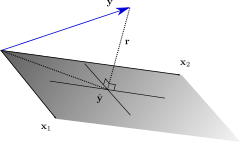
\includegraphics[width=0.6\textwidth]{residu_orth}
	\caption{Illustration of the residual orthogonality in least-squares.}
	\label{fig:pythagore}
\end{figure}


Also an image that is in the \texttt{prebuiltimages/} directory can also be loaded the same way:

\begin{figure}[h] % h stands for here, ! forces even more...
	\centering
	
\includegraphics[width=0.2\textwidth]{umontpellier_logo}
	\caption{Illustration of a prebuiltimage available.}
	\label{fig:umontpellier_logo}
\end{figure}


For displaying side by side some images one should consider the package \lstinline+subcaptions+, that can be loaded with the \LaTeX command:

\begin{lstlisting}[language=tex]
\usepackage{subcaption}
\end{lstlisting}


\begin{figure}[t] % t stands for top (up!)
    \centering
    \begin{subfigure}[b]{0.33\textwidth}
    	\centering
        
\includegraphics[width=0.2\textwidth]{umontpellier_logo}%
        \caption{First example}
        \label{subfig:pythagore}
    \end{subfigure}
    \begin{subfigure}[b]{0.56\textwidth}
    	\centering
        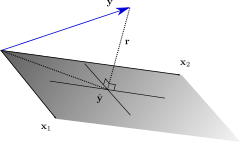
\includegraphics[width=0.5\textwidth]{residu_orth}%
        \caption{Second example}
        \label{subfig:logo}
    \end{subfigure}
    \caption{Exemples of side by side images}
    \label{fig:double_example}
\end{figure}


% ...more text here.
%!TEX root = ../article.tex


%%%%%%%%%%%%%%%%%%%%%%%%%%%%%%%%%%%%%%%%%%%%%%%%%%%%%%%%%%%%%%%%%%%%%%%%%%%%%%%
%%%%%%%%%%%%%%%%%%%%%%%%%%%%%%%%%%%%%%%%%%%%%%%%%%%%%%%%%%%%%%%%%%%%%%%%%%%%%%%
\section{Algorithms}
\label{sec:algorithms}
%%%%%%%%%%%%%%%%%%%%%%%%%%%%%%%%%%%%%%%%%%%%%%%%%%%%%%%%%%%%%%%%%%%%%%%%%%%%%%%
%%%%%%%%%%%%%%%%%%%%%%%%%%%%%%%%%%%%%%%%%%%%%%%%%%%%%%%%%%%%%%%%%%%%%%%%%%%%%%%

Considering the techniques mentioned by \citet{Jaggi13}, you can use a different algorithm a in say \Cref{alg:DC}



{\fontsize{4}{4}\selectfont
\begin{algorithm}[h]  % again h stands for here
\SetKwInOut{Input}{input}
\SetKwInOut{Init}{init}
\SetKwInOut{Parameter}{param}
\caption{\textsc{Implicit differentiation}
}
%
\Input{$
    X \in \bbR^{n \times p},
    y \in \bbR^{n},
    \lambda \in \bbR,
    n_{\text{iter}} \in \bbN$}
    \tcp{jointly compute coef. and Jacobian}

    \If{Lasso}{
    Get $\beta = Lasso(X, y, \lambda, n_{\text{iter}})
    $ and its support $\hat S$.

    $\hat J_{\phantom{\hat S}} = 0_{p}$ 
    \tcp{affectation}

    $\hat J_{\hat S} =
    - n e^\lambda (X_{\hat S}^\top X_{\hat S})^{-1} \sign \beta_{\hat S} $
    }
    \If{wLasso}{
    Get $\beta = wLasso(X, y, \lambda, n_{\text{iter}})
    $ and its support $\hat S$.

    $\hat J = 0_{p \times p}$

    $\hat J_{\hat S, \hat S} =
    - (X_{\hat S}^\top X_{\hat S})^{-1}
    \diag ( n e^{\lambda_{\hat S}}
    \odot \sign \beta_{\hat S})$
    }
\For{$k = 0,\dots, n_{\text{iter\_jac}} - 1$
    }{a = 1}

\Return{$\beta, \hat J$}
\label{alg:compute_jac_implicit_diff}
\end{algorithm}
}


It is also possible to use the standard citation style \cite{Tibshirani96}.


% if needed add appendix here:
% \input{content/appendix}

\newpage
\bibliographystyle{plainnat}
\bibliography{../biblio/references_all}
% see https://github.com/josephsalmon/OrganizationFiles/biblio/references_all.bib, or adapt your own from that one.

\end{document}
